%\documentclass[10pt, journal, final]{IEEEtran}
\documentclass[11pt]{article}
\usepackage{amsmath}
\usepackage{amsthm}
\usepackage{breqn}
\usepackage{graphicx}
\usepackage[T1]{fontenc}
\usepackage{setspace}

%\doublespacing

\newtheorem{theorem}{Theorem}
\newtheorem{mydef}{Definition}

%\usepackage{float}
%\floatstyle{boxed}
%\restylefloat{figure}

\begin{document}

\title{Location Privacy in Cellular Networks}
\author{David Mis}

\maketitle

\begin{abstract}
	Current cell phone networks require constant tracking of customer locations and call metadata, but modern cryptography allows us to design networks that protect the locational privacy of cell phone users. We present a cellular network that does not require constant tracking of a customers location and is able to connect calls without knowing which customers are communicating. This novel network design provides locational privacy using unlinkable pseudonyms. It prevents unauthorized use of network resources through an anonymous credential scheme based on RSA blind signatures. We implemented a prototype network that is largely compatible with GSM using Nexus S Android phones. The prototype demonstrates that our system can easily be run on modern cellular equipment.
\end{abstract}

\section{Introduction}
Cell phones are the most widely adopted consumer technology in history; over 75 percent of the world's population has access to a cell phone and over 90 percent of the world's population is covered by cell phone service \cite{worldbank2012maximizing}. Unfortunately, cell phone networks are forced to track a user's location in order to connect calls. Currently, the only way a person can hope to prevent their movements from being systematically tracked by networks (and consequently telecoms and governments) is to not carry a cell phone. This sort of location tracking is especially dangerous because it is silent, pervasive, and cheap, which opens the door for abuse by law-enforcement, telecoms, and criminals \cite{blumberg2009whitepaper}.

Modern cryptography allows us to build cell phone networks that preserve the locational privacy of their users. In this paper, we propose a new location registration system that allows users to roam and connect calls while preventing any third party (including the network itself) from identifying the owner of any particular phone. Furthermore, we use anonymous credentials based on blind signatures to build an authorization scheme that only allows paying customers to access network resources. Our schemes preserves the locational anonymity of users in the Random Oracle Model, and is largely compatible with existing GSM infrastructure. 

Our system has two main components. The first component is a location register using unlinkable pseudonymic aliases for location registration and call connection. Aliases are constructed using a pseudorandom function that reveals no information to the network that could identify a particular phone, but still allows authorized contacts to call one another.

The second component is an anonymous credential scheme using tickets built with RSA blind signatures. These tickets allow the network to be confident that only paying customers are able to access network resources, but they still prevent the network from identifying the holder of a particular ticket. Although tickets can be transferred, they can not be reused without compromising the locational privacy of the abusing parties.

We implemented the client-side of our system on Google Nexus S Android phones. Our tests show that the anonymity-preserving features put only mild strain on phone resources. Our system introduces no noticable latency for the user and has a negligable affect on battery life.

The rest of this paper proceeds as follows: Section 2 gives a brief overview of related research. Section 3 gives a high-level overview of our proposed system, its design goals, and its threat model. This description is made explicit in Section 4. Section 5 describes and evaluates the prototype network. Our design goals are reexamined in Section 6. Section 7 discusses possible attacks, and Section 8 concludes. Appendix A is a primer on GSM.

\section{Related Work}
The idea of anonymous connections in GSM was first proposed in a scheme by Lin and Jan \cite{lin2001wireless}. Unfortunately, they included a faulty proof-of-security, and \cite{barbancho2003cryptanalysis} subsequently demonstrated that the LJ scheme was insecure. Specifically, the LJ scheme used ticket-based anonymous credentials that could be forged, transferred, and reused \cite{yang2005secure, barbancho2003cryptanalysis}. In this paper, we avoid these pit-falls by using provably unforgeable, one-time-use authentication tickets. Tickets can still be transferred between users, but re-use compromises the offender's anonymity, making it easy for network administrators to detect and identify abusive users (discussed more in Section 4).

Several schemes have expanded and improved the LJ scheme \cite{hwang2006wireless, peinado2004privacy, yang2005secure}. These schemes focus on providing anonymous connections for mobile stations while roaming in a visiting network. In contrast, our scheme provides anonymity for users even when connecting to their home network. It should be noted that we allowed ourselves more freedom in changing a customer's experience when using their phones; where previously proposed schemes only require changes that are transparent to the user, we have added an additional handshake between mobile stations before the first time they wish to call each other (similar to the user handshake found in many VOIP systems like Skype).

There has also been extensive research into the privacy properties of VOIP systems. \cite{wang2005tracking, benini2008assessing} shows how a network attacker could introduce "timing watermarks" into call data in order to identify two communicating parties. Melchor et al proposed a system to solve this issue by introducing dummy messages to make calls unobservable in a system with a limited number of users \cite{melchor2007closed}.  Our paper complements this existing body of work by introducing an address register system that prevents even system administrators from identifying the addresses of particular users. This is especially important in peer-to-peer systems like Skype where the location register is distributed among thousands of untrusted nodes \cite{garfinkel2005voip, perenyi2007skype}. The ideal VOIP system will protect users from identification from inside the system as in our scheme as well as protect against identification from external attackers at call-time like in Melchor et al.

\section{Model}
This section gives a broad overview of our system, its threat model and design goals. 

\subsection{Framework}
Our framework reflects the infrastructure of modern GSM networks. Phones are carried by users as they roam around a network's service area. The phones communicate with cell towers, called Base Station Transceivers (BSTs). A group of BSTs are controlled by a Base Station Controller (BSC), which are in turn managed by a Mobile Switching Center (MSC). The network groups one or more BSTs into a Location Area (LA). Each LA is uniquely identified by a Location Area Identifier (LAI). Each phone belongs to a single LA at a time, and the network need not pinpoint the location of a particular phone beyond its LA in order to connect calls. 

A quick note on terminology: \emph{Network} is used to refer to all parts of the system under a telecom's control --- that is the BSS, MCS's, location registers and so forth. It does not include phones. The distinction between a phone and a Mobile Station (phone + SIM) is not important here, so we use \emph{phone} to refer to what GSM calls "Mobile Station." Likewise, the distinction between HLR and VLR is not important for our purposes, so \emph{location register} refers to a database containing the information that would be spread between HLR's and VLR's in GSM.

Phones identify themselves to the network by presenting an \emph{alias}. Each alias appears to be a random string to the network, and subsequent aliases presented by the same phone are unlinkable. Each phone informs the network of its current position with a message containing its current alias and location area. This process is called "location update," and it is executed whenever a phone enters a new location area or whenever the phone changes its alias.

When a user Alice wants to call her friend Bob, her phone must ask the network to construct a call circuit ending at a phone with Bob's current alias. Although aliases appear random to the network, Alice is able to calculate Bob's current alias so long as she and Bob previously completed a one-time handshake protocol called "alias exchange." Although the requirement that Alice and Bob complete a handshake before connecting calls is a departure from the current cell phone user experience, it is no more involved than procedures already being used by VOIP systems or social media websites.

In order to prevent unauthorized use of network resources by anyone other than paying customers, phones must periodically (about once a month) identify themselves to the network and obtain a number of single-use anonymous credential tickets. These tickets are unforgeable, so the network can verify that each legitimate ticket is the result of a protocol in which it agreed to participate, but no ticket provides any information that could be used by the network to identify a particular ticket-holder. A phone presents the network with a single-use ticket whenever it registers with a new alias. Since a phone must execute the location update protocol before it can make or receive calls, the network is confident that all calls are connected only between authorized parties.

\subsection{Threat Model}
By "attacker" or "adversary" we mean a global passive attacker such as the operator of the network (i.e. phone company) or a government with a total view of the network. If we can defend against this strong attacker, then we can also defend against rogue phone company employees, criminals, or governments with only a partial view of the network. This adversary is \textit{global} since it has a total view of the network including the Base Station Subsystem, all Mobile Routing Centers, and the contents of all databases. The adversary is also \textit{passive}, meaning we assume the attacker will not interfere with the network or operate phones of their own. While it may not be realistic to expect an attacker to refrain from interfering with network traffic in order to compromise users' locational anonymity, a network that is secure against a global passive adversary will require any attackers to expend additional effort and resources to perform attacks against users, so attacks would be more difficult and costly. We relax this assumption and informally discuss active attacks in Section 7.

    We assume:
\begin{enumerate}
\item
An attacker will know the location area (LA) of any phone the moment it transmits data over the network. We make no assumptions about the size of location areas.
\item
An attacker can view all data being transmitted at any point in the network.
\item
	An attacker can indefinitely store (sender location, receiver location, time, data) tuples. "Location" could be a LA of a phone (in the case of call data) or some part of the network itself (such as an MSC).
\item
	Phones transmitting identical messages under identical circumstances (that is, to/from the same location at the same time) are are indistinguishable.

\end{enumerate}

\subsection{Design Goals}

The most important design goal for our network is the following: A user's location should not be revealed as part of normal network usage during MS power-on, location update, sending or receiving calls. Furthermore, a global passive attacker should not normally be able to easily obtain a user's location during normal network usage.

What is meant by "easily obtain a user's location" is admittedly vague and ambiguous. In particular, we are not concerned with the problem of traffic analysis. 

We are also considering the following goals:
\begin{enumerate}
\item
The new network should require only minimal changes to the user's experience. Customers should be able to use their cell phones in a similar way as they can in current GSM networks.
\item
Only authorized users may access the network. There must be some mechanism in place to be sure customers are up-to-date on phone bills without disclosing the identity of any customer using the network.
\item
The new network should be largely compatible with existing infrastructure, so current smartphones and cell towers should work with the new network. In particular, we will focus on updating the software of phones and networks, but try to avoid making significant hardware changes.
\end{enumerate}

We use the following definitions in the theorems in this report:
\begin{mydef}Locational Privacy.
	Let \textbf{S} denote the network's location register database of $\langle alias, (LA_0, LA_1, ...), (time_0, time_1, ...) \rangle$ tuples.

	Let \textbf{S'} denote a database generated from \textbf{S} by removing the alias tuple field -- that is, a database where for every $\langle alias, (LA_0, LA_1, ...), (time_0, time_1, ...)\rangle$ tuple in \textbf{S} there is a corresponding $\langle(LA_0, LA_1, ...), (time_0, time_1, ...)\rangle$ tuple in \textbf{S'}.

	Let \textbf{V} denote all information available to the network servers. This includes all information sent to the server by phones during the \emph{GrantTicket, UpdateAlias, RequestCall} and \emph{\texttt{AcceptCall}} protocols, which includes \textbf{S}.

	Let \textbf{V'} denote all information contained in \textbf{S'}.

	A protocol preserves the \emph{locational privacy} of a user $U$ if the network administrator's information about $U$ is insignificantly larger in \textbf{V} than in \textbf{V'}.
\end{mydef}

Note that the server will still have some information about the number of phones registered in a particular LA based on the information in \textbf{V'}, but it will not have any information about the identity of those phones except possibly that they recently moved to or from a different location area. The registers will have multiple location areas for a single alias only when the phone changes location areas before changing its alias. 

We do not protect against identification of phones based on information outside the system. For instance, if the network knows that Alice has the only phone in a particular location at a particular time, then it can still track her movements.

\section{Architecture}

This section gives a precise descripton of our new cellular network. The protocols are illustrated in Figures 2, 3, and 4.

The system runs over several phases. In order to call one another, users must exchange secrets in the AliasExchange phase. They can then use these secrets to compute each others aliases at call-time using GenerateAlias. At the beginning of each month, a phone must obtain from the network an authorization ticket for each of the aliases it plans on using that month. This happens in the GrantTicket phase. During this phase, the network is able to identify the user, but is not able to later link the tickets it generates to the user. When a phone moves around in the world, it must occasionally execute UpdateAlias in order to be reachable for calls. This phase is akin to location registration in GSM. Finally, calls are initiated during the RequestCall and \texttt{AcceptCall} phases. A phone "dials out" during the RequestCall phase, while incoming call requests are handled in the \texttt{AcceptCall} phase.

The following definition is important for some proofs in this section:
\begin{mydef} Online: Assume that Alice is scheduled to run \emph{UpdateAlias} at times $t_0, t_1, t_2$ etc. By the phrase \emph{"Alice is online"} we mean that if $t_n <= \texttt{current_time} < t_{n+1}$, then Alice has successfully and faithfully run \emph{UpdateAlias} in some location area where she is able to receive incoming call requests.
\end{mydef}

We now present a detailed description of all protocols necessary to locate phones in the anonymous cell network, including anonymous authorization protocols to prevent unauthorized access to the network. All protocols here assume reliable delivery of messages.

\subsection{AliasExchange}
During this phase, Alice and Bob exchange all secrets needed to call each other. The values of \texttt{timingSecret} and \texttt{idSecret} are used to generate aliases for location registration and call requests, while \texttt{sharedKey} is used for end-to-end encryption and authentication. \texttt{$K_Alice$} and \texttt{$K_Bob$} are Alice's and Bob's public keys, respectively. AliasExchange only needs to be executed once for each pair of contacts.

This phase can be done outside our system, such as over the Internet, a USB cable, or an NFC connection between the phones. As such, we do not specify exactly how this phase must be implemented. For instance, \texttt{sharedKey} may be generated through Diffie-Hellman Key Exchange \cite{diffie1976new} or a simpler protocol depending on the environment in which AliasExchange is being executed. 

In order to protect a user's anonymity, all \texttt{timingSecrets} and \texttt{idSecrets} must be unique. If two phones both use the same values for \texttt{timingSecret} and \texttt{idSecret}, then their alias will always be the same. The network can then track the movements of these phones by searching the location register for matching aliases. For theoretical purposes, we assume that a trusted third party generates unique values for all users. The probability that two users out of 10 billion would choose the same random 256-bit values for \texttt{timingSecret} or \texttt{idSecret} is on the order of $8 \times 10^{-58}$, which is probably acceptable in practice.

\subsection{GenerateAlias}
GenerateAlias allows phones to generate cryptographic aliases that appear random to network administrators, but still allow the phone to be reached by anyone who was previously authorized by the phone to do so. This phase not only generates unpredictable aliases, but also generates new aliases at unpredictable times (from the point of view of network administrators). The only restriction is that the time between alias updates can not exceed a \texttt{MAX_TIME} parameter. All aliases older than \texttt{MAX_TIME} can be discarded from the network location registers; otherwise the network would need to store stale aliases indefinitely. 

There are three reasons why random update intervals are preferable over a fixed-interval scheme: first, it prevents all phones from updating aliases at the same time, which would put unnecessary load on the network. Second, with carefully chosen parameters, it will more difficult for network administrators to detect exactly how many phones are in a given location area at any particular time. If all phones update aliases at the same time, then the nework would have a snapshot of exactly how many phones are in each LA every few minutes. Third, it will be more difficult for a network administrator to know if a location update is coming from a phone that is being turned on, moving location areas, or just providing its periodic update. 

This phase is executed as follows: assume we have two phones, Alice and Bob. Each phone has two secrets it must share in order to be reachable for calls---a \texttt{timingSecret} and a \texttt{idSecret}. These secrets are exchanged during the AliasExchange phase. At the highest level, the alias generator is a one-way function $F$ such that:
\begin{equation*}
	F(\texttt{timingSecret}, \texttt{idSecret}, \texttt{current_time}) = \texttt{current_alias}.
\end{equation*}

The generator proceeds in two phases. In the first phase, it determines the last time the alias was updated, \texttt{last_update_time}, based on \texttt{timingSecret} and \texttt{current_time}. In the second phase, the generator produces \texttt{current_alias} based on \texttt{last_update_time} and \texttt{idSecret}. Phones offer \texttt{current_alias} to the network through UpdateAlias at \texttt{last_update_time} and when changing location areas in order to be reachable for calls. Also, phones can initiate an outgoing call via RequestCall by providing the network with the \texttt{current_alias} of a friend. 

The alias generator has several parameters, described below. All times throughout this report are in milliseconds since the start of the UNIX Epoch.

\begin{center}
\begin{tabular}{p{4cm} p{9cm} }
%\texttt{GLOBAL_MAX_UPDATE}: &  
%			The network's timeout for aliases in the location registers. Phones must not have intervals longer than \texttt{GLOBAL_MAX_UPDATE} between alias updates or they may be unreachable. This is the only global parameter; all others can be set individually by phones and shared with friends (although it may be preferable for all phones to share the same parameters to avoid leaking information based on the timing of updates). \\[0.5cm]
\texttt{PERIOD_LENGTH}: &
			A period is a relatively long time frame which provides a reference for computing \texttt{update_time}. In the prototype network, phones set this parameter to 1 day. \\[0.5cm]
\texttt{MIN_UPDATE}: &
			The minimum time between updates. The prototype implementation assumes this is a positive value, but it could be set to 0 with only a few small modifications. \\[0.5cm]
\texttt{MAX_UPDATE}: &
			Th maximum time between updates. \\[0.5cm]
\texttt{UPDATE_GRANULARITY}: & 
			A relatively small length of time that gives the number of possible updates per period. For instance, if we want to allow phones to be ale to update their aliases at any second and we set \texttt{PERIOD_LENGTH} to one day, then \texttt{UPDATE_GRANULARITY} is the number of seconds in one day. 
\end{tabular}
\end{center}

The preceding parameters should all be shared between all phones in the network. If a phone sets its own timing parameters, then it may leak identifying information to the network based on the frequency of its alias updates.

	The first phase proceeds as follows. First, the generator determines the start of the current period, named \texttt{period_start}, by computing 
\begin{equation*}
	\texttt{period_start} = \texttt{current_time} - (\texttt{PERIOD_LENGTH}\; \% \;\texttt{current_time}). 
\end{equation*}
It then produces an array of \texttt{alias_update_scalars} by hashing 
\begin{equation*}
	\texttt{timing_digest} = SHA-256(\texttt{timingSecret}, \texttt{period_start}, \texttt{iteration_number})
\end{equation*}

where \texttt{iteration_number} is incremented for each hash necessary to fill the array. Each digest gives a number of \texttt{alias_update_scalars} by taking successive strings of bits from the digest. The generator can now recursively produce a sequence of \texttt{alias_update_times} by
\begin{equation*}
\begin{split}
\texttt{alias_update_time_1} =  &\;  \texttt{period_start} + \texttt{MIN_UPDATE}  + \\ 
	& (\frac{\texttt{alias_update_scalar_1}}{\texttt{max_alias_update_scalar}}) (\texttt{MAX_UPDATE} - \texttt{MIN_UPDATE}), \\
\end{split}
\end{equation*}
\begin{equation*}
\begin{split}
	\texttt{alias_update_time_n} =  &\;  \texttt{period_start} + \texttt{MIN_UPDATE}  + \\ 
	& (\frac{\texttt{alias_update_scalar_n-1}}{\texttt{max_alias_update_scalar}}) (\texttt{MAX_UPDATE} - \texttt{MIN_UPDATE}), \\
\end{split}
\end{equation*}
	  
where \texttt{max_alias_update_scalar} is the largest possible scalar (ie. for 16-bit scalars, this is 0xFFFF). The size of the update scalars is determined by \texttt{PERIOD_LENGTH} and \texttt{UPDATE_GRANULARITY}. The largest \texttt{alias_update_time} that does not exceed \texttt{current_time} is taken to be the \texttt{last_update_time}, and this concludes the first phase of the generator.

Note that there is one special case. If \texttt{current_time} is less than \texttt{alias_update_time_1}, then the first phase must be repeated using the previous period. This is a relatively rare corner case since it will only happen when a phone tries to make a call in the first few minutes of a period, and it can be detected quickly since \texttt{alias_update_time_1} only depends on \texttt{alias_scalar_1}.
	    
The second phase of the generator consists of a single step: the generator produces \texttt{current_alias} by:
\begin{equation*}
	\texttt{current_alias} = SHA-256(\texttt{last_update_time}, \texttt{idSecret}).
\end{equation*}

\subsection{GrantTicket}
The GrantTicket phase generates authentication tickets. It can be executed infrequently, perhaps once a month. Alice computes all her aliases for the month, identifies herself to the the network, then obtains an RSA blind signature from the network for each of her \texttt{$\langle aliases, update_time \rangle$} tuples. Each of these blind signatures is an authentication ticket and helps the network detect unauthorized access. In order to prevent ticket re-use, a ticket is only valid for a given alias at a given time; Alice could transfer some of her tickets to a friend, but the network could detect abuse if she also tried to use the tickets herself.

Before any phone can execute GrantTicket, the network must generate RSA exponents $d$ and $e$ and modulus $N$, then publish $e$ and $N$. The random value $r$ should be relatively prime to $N$. Furthermore, Alice should check that the network faithfully signed her tickets by verifying $(ticket_{alias})^e$ mod $N = (alias, time)$; the network may be able to link a faulty ticket to a user during location registration if it does not honestly carry out the blind signature protocol (explained in Section 7.2). As long as Alice verifies that the network honestly executes the blind signature protocol, she is confident that her tickets will provide no information about her identity during location registration because of the blinding factor $r^e$.

\subsection{UpdateAlias}
The UpdateAlias phase is run during location registration. Alice provides the network with her current alias, a ticket for that alias, and the identity of a location area to register to. The network verifies that the alias has a valid corresponding ticket to prevent unauthorized network access. That is, it must check that $(ticket_{alias})^e \mod N = (alias, update\_time)$. The network also verifies that the alias in the ticket matches the alias sent in the clear by the user, and that the current clock time is within the interval $[update_time - \epsilon, update_time + \texttt{MAX_TIME} + \epsilon]$ where $\epsilon$ is a small positive value that allows for small discrepencies between the phone's and network's clocks. This interval is sufficiently large to avoid erroneously preventing access to legitimate users who are turning on their phones or changing location areas.

\begin{theorem}
	The network will update the location register with Alice's current alias if Alice faithfully executes the \emph{GrantTicket} and \emph{UpdateAlias} phases.
\end{theorem}
\begin{proof}
The network updates the location register if 
\begin{equation*}
	(ticket_{alias})^e \mod N = (alias, update\_time).
\end{equation*}
If Alice faithfully executed the GrantTicket phase, then
\begin{eqnarray*}
	(ticket_{alias})^e \mod N & = & (((alias,current\_time)r^e)^d \times r^{-1})^e \mod N \\
	& = & ((alias,current\_time)^dr \times r^{-1})^e \mod N \\
	& = & (alias,current\_time)^{ed} \mod N \\
	& = & (alias, current\_time) \mod N.
\end{eqnarray*}
\end{proof}

\begin{theorem}The \emph{UpdateAlias} phase preserves the user's locational privacy in the Random Oracle Model.
\end{theorem}

\begin{proof}
	We want to show that network administrators gain no information besides the fact that some phone is requesting to register in a location area; the administrator gains no identifying information about the phone. During the UpdateAlias phase, a user sends the four pieces of information to the network backbone: a string \texttt{UPDATE_ALIAS}, the user's current alias, a ticket for the user's alias, and the location area to register the alias. None of these fields reveal any information about the user:

\texttt{UPDATE_ALIAS} is a fixed string used by all users to request updates to the location registers.

From the backbone's point of view, \texttt{alias} is indistinguishable from random in the Random Oracle model since it is the result of \texttt{SHA-256(last_update_time, idSecret)} in GenerateAlias.

The network is able to verify that the ticket corresponds to the provided alias and was signed during the GrantTicket phase, but since the signature was blinded with random blinding factor $r^e$, the network is not able to link the ticket with any particular users or operations it performed during the GrantTicket phase.

\texttt{LA} does not reveal any identifying information about the user since every user who wishes to register to the same location area must use the same \texttt{LA} value.
\end{proof}

Using tickets based on RSA blind signatures limits unauthorized network access. These signatures are unforgeable, so a ticket can only be created during the GrantTicket phase. A phone could still attempt to register to a location area by borrowing (or stealing) tickets from a legitimate user, but they will only be able register with the corresponding alias at the corresponding time. If multiple phones repeatedly register with the same alias at the same time, then their anonymity is compromised, thus the network will be able to detect unauthorized registration. Even if the attacker steals tickets from many legitimate users, the network will quickly be able to detect unauthorized access since legitimate alias collisions are so rare.

\subsection{RequestCall}
Alice executes the RequestCall phase when she wants to call her friend \texttt{Bob}. The network first verifies that a phone with $alias_{Alice}$ is registered in the current location area to prevent unauthorized access.

If Alice is properly registered, the network will send an incoming call request to all phones registered with alias $alias_{Bob}$.

The values $r$ and $K_{sharedKey}(r)$ are used by the network during the \texttt{AcceptCall} phase to authenticate Bob, and $K_{Bob}("Alice")$ is used by Bob to identify Alice. 

We expect only one phone to be registered with $alias_{Bob}$ at any one time. A small number of collisions are theoretically possible, but highly unlikely. If the network has $L$ unique phones online at any time, we treat SHA--256 in the GenerateAlias phase as a random oracle, and all phones have a unique \texttt{timingSecret} and \texttt{idSecret}, then the probability of a collision at any one time is about $1 - e^{-L^2/2^{256}}$. For L = 10 billion registered phones, the probability of a legitimate collision at any given time is about $4 \times 10^{-58}$. Even if all aliases were updated every millisecond, we would not expect a legitimate collision for many millennia. The network should treat all alias collisions as signs of either attempted unauthorized access or malfunctioning equipment.


\subsection{AcceptCall}

If Bob is online and Alice executes RequestCall, then Bob will receive an incoming call request consisting of \texttt{INCOMING_CALL}, $K_{Bob}(“Alice”)$, $alias_{Alice}$, and $K_{sharedKey}(r)$. In the \texttt{AcceptCall} phase, Bob verifies that he is the intended recipient by decrypting $K_{Bob}(“Alice”)$ and checking that he recognizes the contact. If the decryption is gibberish, then the call is not intended for Bob and the request is the result of a temporary alias collision. He also verifies that an attacker is not impersonating Alice by checking that Alice's current alias returned from GenerateAlias is the same $alias_{Alice}$ received in the incoming call request. An attacker could only register using $alias_{Alice}$ (and thus make a call using this alias) if he was able to execute UpdateAlias using stolen (or borrowed) tickets. Thus Bob can trust the stated recipient in the incoming call request is really Alice as much as he trusts Alice to keep her tickets secret. 

Bob can choose to answer the call by sending the network the decryption of the random tag $r'$.  As long as Bob protects his secret key $K^{-1}_{Bob}$, the network is confident that it is connecting a call between the correct recipients; that is, the receiver is not simply impersonating Bob.

\begin{theorem}
	\emph{RequestCall} and \emph{AnswerCall} respect the sender's and receiver's locational privacy.
\end{theorem}
\begin{proof}
	All messages in these phases are either constants (\texttt{REQUEST_CALL}, \texttt{INCOMING_CALL}, and \texttt{ANSWER_CALL}), random ($r$), or indistinguishable from random from the network's perspective.
\end{proof}								
We have not yet discussed how calls are connected. In a GSM-like system, the network creates a circuit between two channels on BTS's near Alice and Bob. If location areas contain more than one BTS, then Alice and Bob will both have to choose a BTS with strong signal near them and notify the network of these BTS's. This can be done as part of the \texttt{CALL_REQUEST} and \texttt{CALL_ACCEPT} messages, so no additional identifying information about Alice or Bob is required.

In a VOIP system like our network prototype, Alice and Bob must exchange additional sensitive information in order to establish a RTP session, namely IP addresses and open ports. Our prototype is designed so that Alice and Bob can establish the RTP session outside the network's control, thus all sensitive information can be encrypted such that only Alice and Bob are able to read it. This extra encrypted information is sent along with the \texttt{CALL_REQUEST} and \texttt{CALL_ACCEPT} messages. In this way, no additional information is revealed to the network and call connection maintains the locational privacy of Alice and Bob. 

%\section{Discussion}
%We have some flexibility in choosing values for the five parameters. For the prototype network. We set the following parameter values:

%\begin{center}
%\begin{tabular} { l  l }
%	\texttt{GLOBAL_MAX_UPDATE} &= \texttt{MAX_UPDATE} = 10 minutes, \\
%	\texttt{MIN_UPDATE} &= 1 minute, \\
%	\texttt{PERIOD_LENGTH} &= 1 day, \\
%	\texttt{UPDATE_GRANULARITY} &= 1 second.
%\end{tabular}
%\end{center}

%The number of \texttt{alias_update_scalars} that the generator must produce is based on \texttt{PERIOD_LENGTH} and \texttt{MIN_UPDATE} since there must be at least enough scalars to fill a period even if every update happens after \texttt{MIN_UPDATE} milliseconds. If a user wishes to set \texttt{MIN_UPDATE} to 0, then the generator will need to produce scalars until it finds an \texttt{alias_update_time} that exceeds \texttt{current_time}. Our current implementation does not operate this way, but this would be an easy modification. 

%The number of bits needed per scalar is determined by the \texttt{UPDATE_GRANULARITY} and the difference between \texttt{MAX_UPDATE} and \texttt{MIN_UPDATE}. Using the above parameter values, scalars are 16 bit values, and at most 90 hashes must be computed to find a alias\footnote{The true worst case is 92 hashes if \texttt{current_time} falls at the very beginning of a period.}. On a Nexus S Android phone, an unoptimized generator consistently computes an alias in less than a tenth of a second, so even performing hundreds of hashes at call-time will be unnoticeable to a user.


\section{Implementation}
We built a prototype network implementing our new network design. Its main components are a client app running on Nexus S Android phones and a server program running on a laptop. Phones running the client app connect to the serve to build authentication tickets, update their location, and request calls. All protocols are implemented as outlined in Section 4. This section describes the prototype network with special attention given to the areas where it differs from a full-scale cellular networks. We also present an experimental analysis of key performance metrics.

\subsection{Prototype Description}
The network is built on a single laptop. Since we are only concerned with location tracking and authorization protocols. We did not simulate the BSS or SS7 network connecting MSCs. Instead, the network component only contains a location register and authorization mechanisms, which are all that are necessary to implement the protocols in Section 4. When a user wants to make a call, her phone queries the location register for all information necessary to establish a Realtime Transfer Protocol (RTP) session between itself and the intended receiver.

The client app randomly generates all secrets shared between phones at startup time. All phones use the same seed for their PRNG, so secrets are consistent across phones. In a full-scale network, each phone must generate its own secrets in some secure manner and share only with other phones that it trusts.

Before a phone can update its location with the network register (and thus make and receive calls), it must execute the GrantTicket protocol to obtain authorization tickets from the network. When the client app starts, the phone initiates a TCP session with the network program.  The phone then generates its aliases for the next 24 hours, blinds the (alias, time) tuples, and sends them all to the network at once. Once the network has received the batch, it begins signing and returning each ticket, which the phone can then unblind and store for the day.

Before the batch operation begins, the network sends it's RSA public key (N, e) to the phone. In a real system, there must be some mechanism for the phone to be confident this same key is being used by all other phones in the system; if the network crafts different keys for different sets of users, then it will be able to determine which set a user belongs to when it attempts to decrypt the ticket during the UpdateAlias phase. This could be avoided by having the key posted publicly at a well-known location instead of being supplied by the network during the GrantTicket phase.

Once a phone has its authorization tickets for the day, it immediately executes UpdateAlias and is now fully online. The phone also executes the UpdateAlias protocol whenever its alias changes, on average once every 5.5 minutes. Instead of a LAI, a phone's location is modeled as an IP address. This method clearly compromises some of the phone's locational privacy, but this would not be an issue in a full-scale cellular network. If we were to adapt our prototype into a fully deployed VOIP network, we could hide each phone's IP from the location register using a mixnet such as TOR \cite{dingledine2004tor, goldschlag1999onion}. Note that only communication between phones and the network needs to be funneled through the mixnet, not communication between phones. This way, we avoid unacceptable mixnet-induced latency of call data. 

Call data is sent over an RTP session between two phones; it is not funneled through the network program on the laptop as it would in a full-scale cellular network since this would introduce unnecessary delays. When a user wants to make a call to an online friend, her phone first begins an RTP session and by opening an RTP port and an RTP Control Protocol (RTCP) port in compliance with RFC 3550 \cite{schulzrinne2003rfc}. It then executes the RequestCall protocol as explained in Section 4.5, but it also informs the network of its RTP port (the RTCP port is always one port higher). If the network finds the requested recipient's alias, it begins the AcceptCall protocol. Once the receiver is informed that a call is incoming and the user chooses to answer, the receiver generates its own pair of RTP ports. Its RTP port is sent along with its response to the caller's challenge in the last message of the AcceptCall protocol illustrated in Figure 3. Once the receiver authenticates, the network sends each phone its peer's IP address and port numbers so they can connect the RTP session and the users can begin talking to each other. This last step is not necessary in a full-scale network that handles call traffic itself.

\subsection{Performance}

We tested our system on Nexus S Android phones running Android version 4.1.1 with 1 GHz single-core ARM Cortex-A8 processors and 512 MB RAM. 

Generating aliases for location update and call initialization happens too quickly to be noticeable by a user. To demonstrate this, we generated 1000 aliases each using fresh, random secrets. The median time to generate a single alias was 25 ms, with 99 percent of aliases being generated in less than 68 ms. The longest observed time to generate a single alias was 312 ms.

Our prototype took substantially longer to generate authorization tickets. We generated several sets of authorization tickets for aliases generated with fresh, random secrets. We chose parameters so that we expect the phone to update its alias every 5.5 minutes, meaning we expect to need to generate about 260 tickets per day. The total time needed to execute GrantTicket and obtain a set of tickets ranged from about 18 seconds for a single day's worth of tickets to 7.8 minutes for a month's worth. On average, 87 percent of the time was due to the phone's cryptographic calculations, with the remaining 13 percent shared between communication with the network and the network's signing operations.

\begin{figure}[h]
\caption{Time to generate batch of tickets.}
\centering
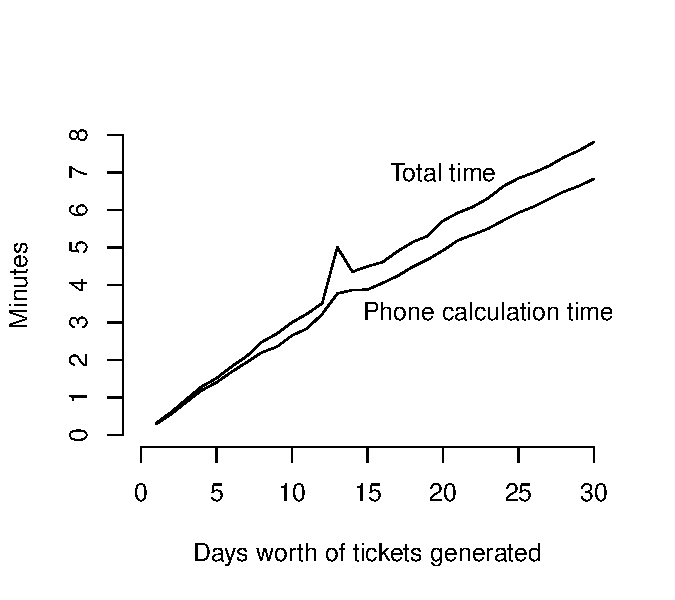
\includegraphics{GrantTicketTime.pdf}
\end{figure}

We also investigated the relative power-consumption of our UpdateAlias protocol. Since phones must execute this protocol both when it changes LA and when its alias changes (as opposed to only when updating LA like in GSM), we expect our system to drain a phone's battery faster than current GSM networks. To test this. We ran the phone app and recorded the phone's battery level every five minutes. The average time between alias updates was 5.5 minutes. We repeated this test without running the phone app at all and compared the difference in battery level. Both tests were run with the screen on full brightness for the duration of the test, and the screen displayed the Android "Settings" menu. After 30 minutes. We detected no difference between the phone's charge levels (both started at 94\% charge and ended at 89\% charge). A more strenuous test may detect increased power consumption while running the UpdateAlias protocol, but this simple test shows the difference is probably small.

We may also be interested power-consumption during the GrantTicket phase. Since this is a computation- and communication-heavy protocol that takes a relatively long time to complete, we expect it to have a measurable affect on the phone's power consumption. However, this operation can be executed so infrequently that it should normally only occur while the phone is charging anyways, so we did not investigate its power-use.

\section{Evaluation}
In this section. We evaluate our network design in regards to the design goals enumerated in Section 3.3. 

We fulfilled our primary goal -- to prevent a user's location from being revealed to the network during normal operation -- through the use of unlinkable, anonymous aliases. All communication between phones and the network are handled with these aliases except possibly during the beginning of the GrantTicket protocol when a user may have to fully identify herself as a paying customer in order to build authorization tickets. This protocol only needs to be executed infrequently, such as once per day, per week, or per month depending on how many 128-byte tickets a phone is willing to store. If this infrequent breach of locational privacy is unacceptable for a user, then she could set up a proxy to execute the protocol for her, such as a home computer. Her phone could then obtain the tickets from the proxy without the network's knowledge.

We also considered several secondary goals. First, we wished to limit differences in the user's experience between our system and existing cellular networks. We were not completely successful here; users can only call other users with whom they previously executed AliasExchage. While this is certainly different from current networks, it is not a completely alien idea to anyone who has used VOIP systems like Skype. AliasExchange can be executed completely outside our network design, so users and other designers can build the methods that work best for them. For example, phones could exchange alias information over Near Field Communication (NFC) simply by touching phones together in phones equipped with such technology, such as the Galaxy Nexus. Another option is an anonymous bulletin system built over the internet where users could post alias information for one another. Any system built on our network design will need to incorporate a method for executing AliasExchange that is acceptable to its users.

Some users in an anonymous alias network, such as customer-service lines, may want to be accessible to all users without first executing AliasExchange. If they are not concerned with location tracking, then such parties could simply publish their identity and timing secrets for everyone to see. This is probably acceptable for call-centers and businesses whose location is public information anyway. An employee's phone could even advertise two sets of aliases -- one for their personal line and one for the business line. If the alias generating secrets of their business line are publicly available, then their location privacy will be compromised, but the phone could simply stop executing UpdateAlias outside of business hours. A final consideration for a deployed network is emergency services such as Enhanced 911. No user who calls 911 will want to keep their location secret from emergency services, so emergency calls must be handled as a special case.

We also attempted to limit network access to only paying customers. We accomplished this by using anonymous credentials based on RSA blind signatures. These tickets can be transferred from one user to another, but they can not be reused without the network detecting abuse. Furthermore, tickets are only valid for a particular alias at a particular time, so even if Alice wants to give some tickets to Bob, Bob would need to tell his friends to use Alice's alias generating secrets when they try to call him. In this sense, our authorization scheme limits an attacker's options to what is already allowed in GSM by transferring SIM cards. Alice can lend her SIM to Bob for him to use in his phone, but Bob's friends would need to dial Alice's number in order to reach Bob. Furthermore, Alice could not access network resources while Bob has her SIM, just as Alice could not access network resources in our system once she gives her tickets to Bob without the network being able to track their locations.   

Finally, we tried to minimize any necessary changes to existing cellular hardware. On the network side, no hardware change is necessary; we simply changed the operation of existing location registers. There will be increased network traffic load from two sources: phones executing GrantTicket and the increased number of location updates due to periodic alias changes. While these changes may require updating old infrastructure, it should be noted that GrantTicket is trivially parallelizable since each ticket is generated independently of all others.

Our system requires no change in phone hardware. Our prototype shows modern phones (the Nexus S was released in 2010) can easily handle our system, albeit with reduced battery life, but we do not know how older phones would perform in the new system. 

\section{Security Analysis}
In this sectio. We drop the assumption that the network is a passive attacker and briefly discuss active attacks against our system that could compromise a user's locational privacy.

\subsection{Compromised Phones}
If the network is able to obtain a user's alias-generating secrets, then it can uncover all the user's aliases and track her movement. For this reason, network administrators should not be able to call customer's cell phones since this would imply they are able to generate the phone's aliases. If administrators need to contact a specific user, there must be an out-of-band method to do so.

Because the security of the system depends entirely on protecting alias-generating secrets, they should be guarded like any other sensitive information on a phone, such as credit card and social security numbers entered into mobile browsers. Alias-generating secrets may be more difficult to protect since a single phone may store dozens or hundreds of friends' secrets, thus an attacker who compromises a single phone will be able to track multiple users. Furthermore, there is a moral hazard problem: friends are not necessarily incentivized to protect their contacts' secrets. However, there is one factor that mitigates the risk of compromise, which is that alias-generating secrets are worthless to an attacker if they do not also have access to the network's location registers, thus they will likely be a less attractive target than credit card numbers or SSNs.

\subsection{Dishonest GrantTicket Implementation}
The network may be able to link an authorization ticket at verification time to a subset of users if it dishonestly executes the GrantAlias protocol. Instead of signing the user's message by raising it to the private key $d$, the network could sign with a different number $dx \neq d$, thus producing a $badTicket$ after the user's phone tries to unblind:

\begin{eqnarray*}
	badTicket & = & (((alias,update\_time)r^{e})^{dx})r^{-1} \mod N \\
	& = & (alias,update\_time)^{dx}r^{x-1} \mod N 
\end{eqnarray*}

This corrupted ticket will not pass the verification check during UpdateAlias, but if the network can reliably check that the verification failed not because of a dishonest user, but instead because the network signed the ticket with $dx$ instead of $d$, then the network can link the phone currently running UpdateAlias to a phone that ran GrantAlias. Since users normally must identify themselves before GrantAlias, this link compromises the user's identity.

The network attempts to decrypt $badTicket$ during UpdateAlias in the following manner. The network attempts to construct the desired ticket $m = (alias,update\_time)$ using the alias sentby the user in the clear and a guess for $update\_time$. If the network guesses $update\_time$ correctly, then it can discover the user's blinding factor $r$:

\begin{eqnarray*}
	(badTicket \times (m^{-1})^{dx})^{(x-1)^{-1}} & = 
	& (m^{dx}(m^{-1})^{dx}r^{(x-1)})^{(x-1)^{-1}} \\
	& = & (r^{(x-1)})^{(x-1)^{-1}} \\
	& = & r \\
\end{eqnarray*}

Once the network has $r$, it tries to use it to recover $(alias, update\_time)$ from $badTicket$.

\begin{eqnarray*}
	((r^{-1})^{(x-1)}badTicket)^{ex^{-1}} & = 
	& ((r^{-1})^{(x-1)}(m^{dx}r^{(x-1)}))^{(ex^{-1})} \\
	& = & (m^{dx})^{ex^{-1}} \\
	& = & m \\
\end{eqnarray*}

If the network recovers $(alias, update\_time)$ at the end of this process, then it knows it built $badTicket$ using $dx$ instead of $d$. If the network fails to recover $(alias, update_time)$, then it may repeat this process with another exponent or another guess for $update\_time$. If none of its exponents work, then the ticket was forged by the user. In this manner, the network could partition users into subsets based on which exponents $x$ it uses to build tickets during GrantTicket.

The most challenging aspect of this attack is guessing $update\_time$. However, since $update\_time$ will normally be close to the current clock time and \texttt{UPDATE_GRANULARITY} limits potential valid times to, say, one or two per second, the network may only need to make a few hundred guesses before stumbling on on the correct value.

Users can detect this attack by checking if $ticket^e \mod N = (alias, update\_time)$ during the GrantTicket phase.
\section{Conclusion}

In this paper, we presented a novel design for a location register for use in cellular networks that protects the location privacy of its users. The security of the system is built on unlinkable anonymous aliases and anonymous credentials that prevent a cellular network from identifying individual users but still allows telecoms to be confident that only paying customers have access to network resources. Our prototype network implementation demonstrates that our scheme can be efficiently realized on modern cellular hardware.

\appendix

\section{GSM Preliminaries}

In order for our anonymity-preserving cellular network to be practical, it must be at least somewhat compatible with existing cell phone infrastructure. That way, existing infrastructure can be reused by anonymity-preserving protocols. This chapter describes modern cellular networks. 

GSM networks are the most common cellular networks in use today. Their protocols are publicly available and open source, and a large body of literature makes them relatively easy to understand. For these reasons. We concentrate on GSM networks in this chapter. We give an overview of the infrastructure and describe the fundamental protocols necessary for connecting calls: registration, location update, incoming call, and outgoing call. We focus primarily on network-level protocols and above; while there are hundreds of lower-level protocols depending on resource constraints and communication endpoints, they are outside the scope of this project. 

\subsection{Infrastructure Overview}
This section gives a brief overview of the main infrastructure of GSM. Each cell phone has a Subscriber Identity Module (SIM card). SIM cards contain all data used to identify and authenticate a user to the network, and it also allows subscribers to easily switch between different phones. Together, a SIM card and cell phone are known as a Mobile Station (MS).  

Cell phone towers are called Base Transceiver Stations (BTS). Each BTS is in the center a hexagonal cell, and is solely responsible for communication to and from all MSs in that cell. Each cell is assigned to a Location Area (LA). Multiple cells may belong to a single LA, and LAs are uniquely identified by a Location Area Identifier (LAI). BTSs are essentially large transceivers and are not equipped to participate in any protocols above the the data-link layer. Instead, multiple BTS in an area are controlled by Base Station Controllers (BSC) that participate in all networking protocols and communicate with the rest of the network. Together, BTSs and BSCs are collectively called the Base Station Subsystem (BSS). 

Network level protocols, such as call routing, are handled by a Mobile Switching Center (MSC). A large network may have multiple MSC, each one responsible for a specific geographic area, but a GSM network may very well have only a single MSC. A special MSC, called the Gateway MSC (GMSC), is the interface between a GSM network and other telephone networks, such as landline networks.  

MSCs are organized into an Signalling System 7 (SS7) network. SS7 is an out-of-band network routing protocol designed for modern telephone systems to quickly establish calls. It is used by most modern landline networks as well as cellular networks. Signals are network control messages as opposed to user-data messages. The protocol is out-of-band, meaning sends signals over a different set of links than links used for user data. The SS7 protocol allows an MSC to discover the current MSC region for any MS given that phone's MSISDN (phone number).

User data is stored in two types of databases: the Home Location Register (HLR) and Visitor Location Registers (VLRs). There is only one HLR per network, and it stores all subscriber's billing and location data. An MSC queries the HLR when it needs to locate a MS in order to complete a call. 

In contrast to the HLR, there can be multiple VLRs (generally one per MSC), each one responsible for tracking all phones in a particular area. They cache much of the same data as the HLR; however, they store more precise location data for each MS. This allows the HLR to only keep track of which VLR is responsible for a particular MS instead of being constantly updated with small changes to the precise locations of each MS. When the HLR needs such precise location data, it queries the appropriate VLR.

GSM also has two additional types of databases. The Equipment Identity Register (EIR) stores information on phones as opposed to users. This allows the network to flag broken or obsolete MSs and refuse service to any MS reported stolen. Another database, the Authentication Center (AUC), stores all cryptographic information necessary to authenticate users and encrypt data in transit. Note that GSM attempts to provide confidentiality against eavesdroppers outside the network, but it does not attempt to prevent network administrators from learning the contents of data sent over the network. That is, GSM does not by default provide end-to-end encryption of customer call data. %Citation?

%Figure “GS. Infrastructure Overview”  illustrates the main components of GSM infrastructure.

\subsection{Registration}
What happens when Alice turns on her brand-new cell phone for the first time?. In order to make or receive calls, Alice's MS must register with the network. To do this, the MS listens for the strongest signal from a nearby BTS, then sends a registration request along with her identity (IMSI) to that tower. The BSC controlling this BTS forwards this information its MSC which then attempts to authenticate Alice's identity using a secret shared between the AUC and Alice's SIM card. If Alice is a subscriber in good standing and her MS is able to authenticate successfully, then the MSC updates the HLR and VLR with Alice's current location. Alice's current VLR is stored in the HLR, and her current LA is stored in the VLR. Additionally, the VLR issues Alice's MS a Temporary Mobile Subscriber Identity (TMSI). This is a temporary alias known only to Alice and the VLR of her current MSC region. Furthermore, this new identifier is used in all communication between Alice's MS and the network. This provides confidentiality against eavesdroppers by protecting Alice's permanent identity, her IMSI. 

\subsection{Location Update}
What happens when Alice drives across the city with her phone on? Each BTS belongs to a LA, and repeatedly broadcasts its LAI over its Broadcast Control Channel (BCCH). Alice's MS monitors these channels, and issues a location update request when it notices that it has crossed into a new LA. This allows the network to maintain the approximate locations of all MS in the network. A location update request is similar to a registration request, but instead of sending its permanent IMSI, Alice's MS identifies itself to the network using its current TMSI. The network updates Alice's current LAI in her current VLR, and issues Alice a new TMSI.

The location updating procedure is executed each time Alice enters a new LA, or possibly intermittently after an interval set by the network. This interval is continuously broadcast over the BCCHs along with each LAI. Furthermore, if Alice travels to a new LA in a different MSC region, then the new MSC will not have Alice's current TMSI stored in its VLR. Since TMSIs  are only valid within a single MSC region, the new VLR will have no way to identify Alice from her TMSI alone. Thus a simple location update is not possible. In this case, either Alice's MS must repeat the registration procedure at her new MSC region, or Alice's new VLR can query her old VLR for her permanent identity (IMSI). This is possible because Alice's MS sends her old LAI along with each location update request, so her new VLR is able to determine her old MSC region and query her old VLR for the TMSI-to-IMSI mapping. 

\subsection{Incoming Call}
What happens when Alice's mother tries to call her? Assume Alice's mother is calling from a landline, so her phone is outside Alice's GSM network. After Alice's mother dials her daughter's phone number, the GMSC receives an IAM connection request signal from outside the network containing Alice's phone number (MSISDN). Because the GMSC is the single access point for all calls terminating in another network, the network needs to establish a connection between the GMSC and Alice's MS. To do this, the GMSC queries the HLR to obtain Alice's current Mobile Subscriber Routing Number (MSRN), which will identify her current MSC region. The HLR either stores the MSRN directly, or it may store Alice's current VLR which it can query to obtain the MSRN. Once the GMSC has Alice's MSRN, a circuit through the SS7 network between the GMSC and Alice's MSC is established. It is now the MSC's responsibility to locate Alice, authenticate her, notify her a new call is incoming, and connect the call if she answers. First, the MSC locates Alice by querying its VLR to obtain Alice's TMSI. The TMSI identifies her current location area, so the MSC instructs the BSC controlling that LA to have all BTSs in Alice's LA broadcast a paging request with her TMSI. Once Alice's MS responds to the paging request, the network identifies Alice's current cell, thereby finishing the phone location procedure. After Alice's MS responds to the paging request, the network must authenticate Alice's identity. Furthermore, all data exchanged between Alice and the network is encrypted over the air (Um interface). At this point, the network is able to route the call between Alice's MS and her mother's landline phone through the GMSC. Alice's MS acknowledges to the MSC that it recognizes an incoming call and starts ringing. If Alice answers, then it notifies the MSC and the call is connected.

\subsection{Outgoing Call}
What happens when Alice tries to call her friend Bob? 
To initiate the call, Alice dials Bob's number on her MS. Regardless of whether Bob is in Alice's same network or not, the network needs to make a connection between Alice's MS and the SS7 interface of her current MSC. Alice's MS first sends a call connection request to her MSC along with her current TMSI, but it does not include the phone number that Alice just dialed. First, the network authenticates Alice and begins a new encrypted session. Only afterwards does Alice's MS transmit the desired number to be called to the MSC. The MSC can then form an IAM signal to be sent over the SS7 network. When Bob is found, the MSC will be notified by an ACM signal from the SS7 network, and if Bob answers, then the MSC is notified by an ANS signal. The MSC then instructs the BSS to connect Alice's call and the two can begin talking.

\subsection{Authentication}
How does GSM authenticate Alice?
GSM needs to authenticate Alice several times over the course of normal cell phone use: at registration, location update, incoming call, and outgoing call. All authentication is based on a secret key $K_{i}$ shared between the network and each MS. The network stores a $K_{i}$ for each subscriber in the AUC, and each MS stores its $K_{i}$ in its SIM. Should Alice's $K_{i}$ become known to an attacker Eve, then Eve could impersonate Alice to the network. 

GSM uses a rather straightforward challenge-response protocol for authentication. Whenever Alice needs to prove her identity, the network presents here with a fresh random number RAND. Alice's MS and the network separately calculate a Signature Response (SRES) based on her $K_{i}$ and RAND using the one-way A3 algorithm. This algorithm was insecure for many years, but its most recent implementation is based on AES. Alice's MS submits her SRES to the network which compares the two values. If they match, then the network declares the authentication successful, and it declares authentication a failure otherwise. To avoid transmitting any subscriber $K_{i}$, all SRES calculations by the network are done at the AUC. A batch of (IMSI, RAND, SRES) tuples are sent by the AUC to any VLC that requests them. The VLC can then challenge any subscriber with RAND and compare their response to SRES without ever knowing $K_{i}$. Each tuple must only be used once to avoid replay attacks. Note that the GSM authenticates Alice, but Alice does not authenticate the network. This allows anyone with the right transceivers to impersonate Alice's network and potentially steal sensitive information.


\bibliography{bibliography}
\bibliographystyle{plain}

\begin{figure}[p]
	\caption{Illustration of AliasExchange, GrantTicket, and UpdateAlias phases.}
	\centering
	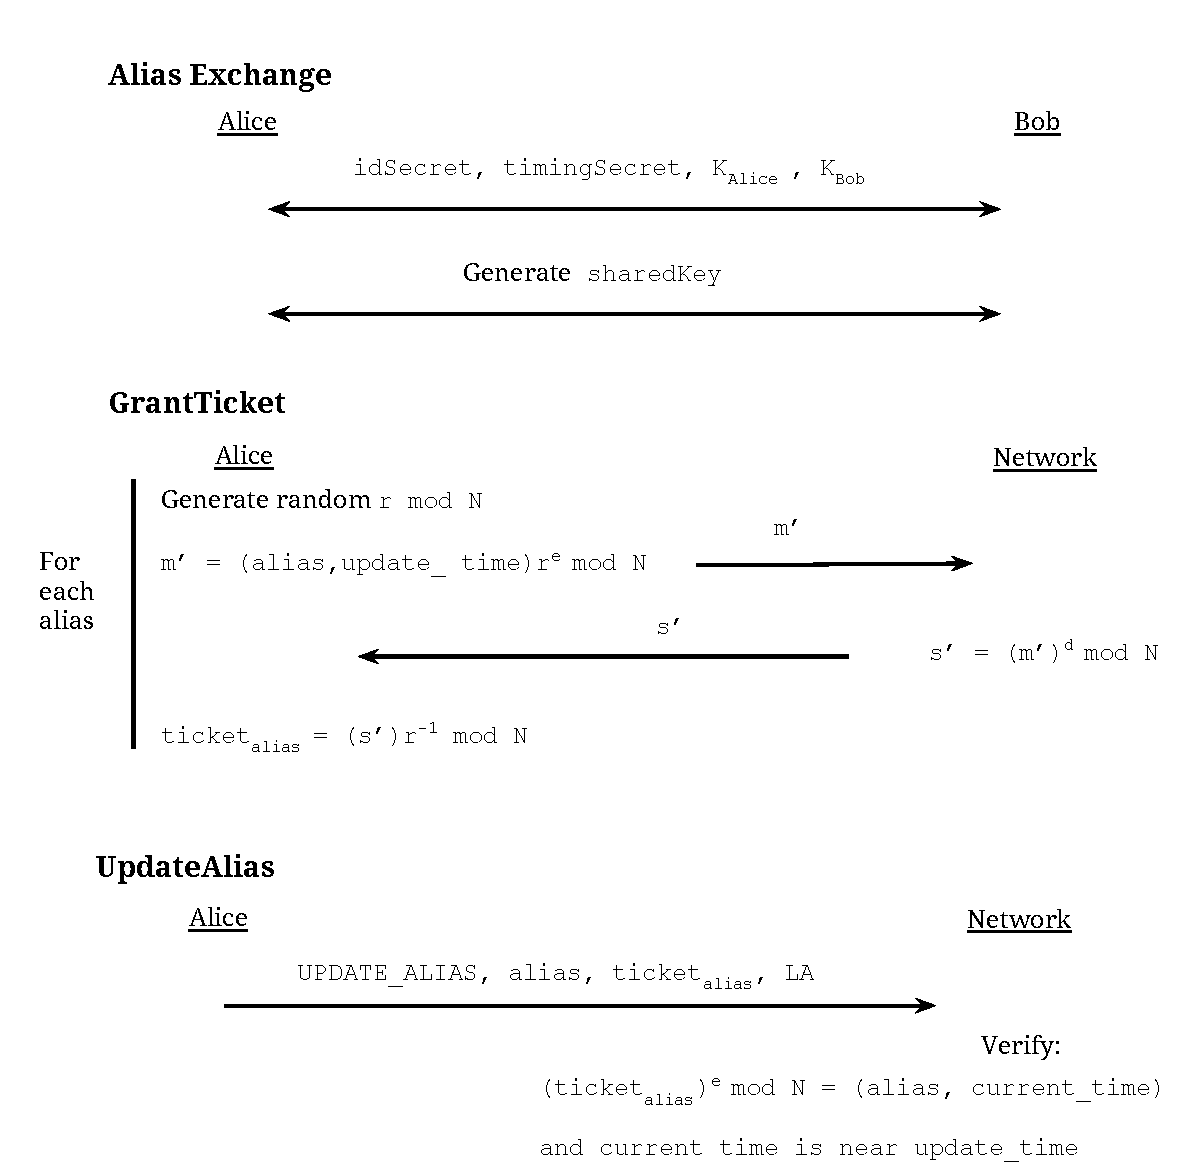
\includegraphics[scale=0.65]{ProtocolsIllustration.pdf}
\end{figure}

\begin{figure}[p]
	\caption{Illustration of RequestCall, and AnswerCall phases.}
	\centering
	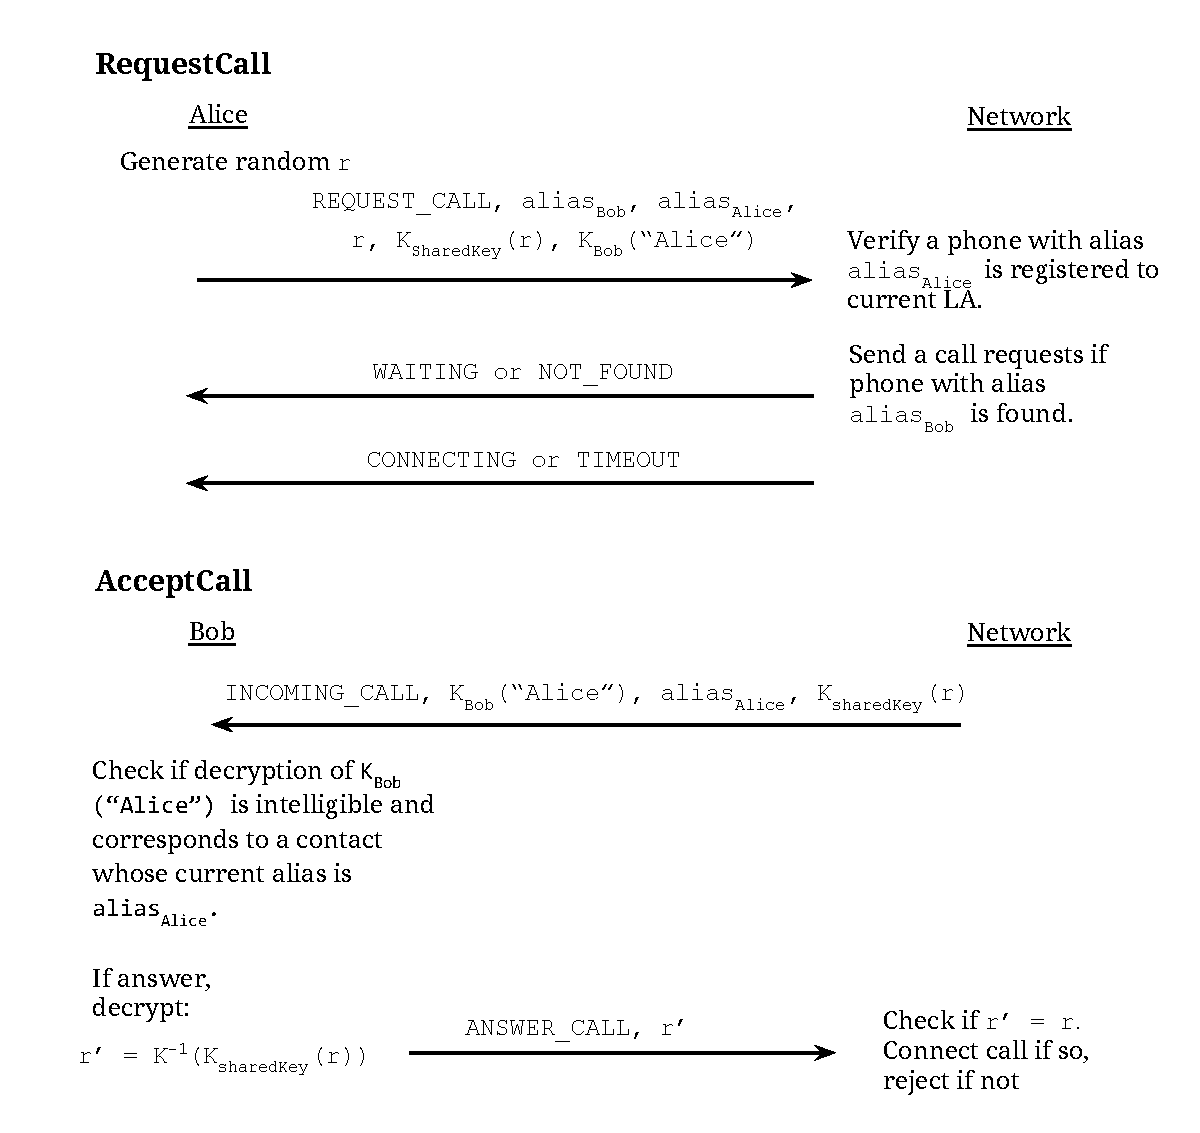
\includegraphics[scale=.65]{ProtocolsIllustration2.pdf}
\end{figure}

\begin{figure}[p]
	\caption{GenerateAlias. In this figure, Bob is computing Alice's current alias in order to make a call.}
	\centering
	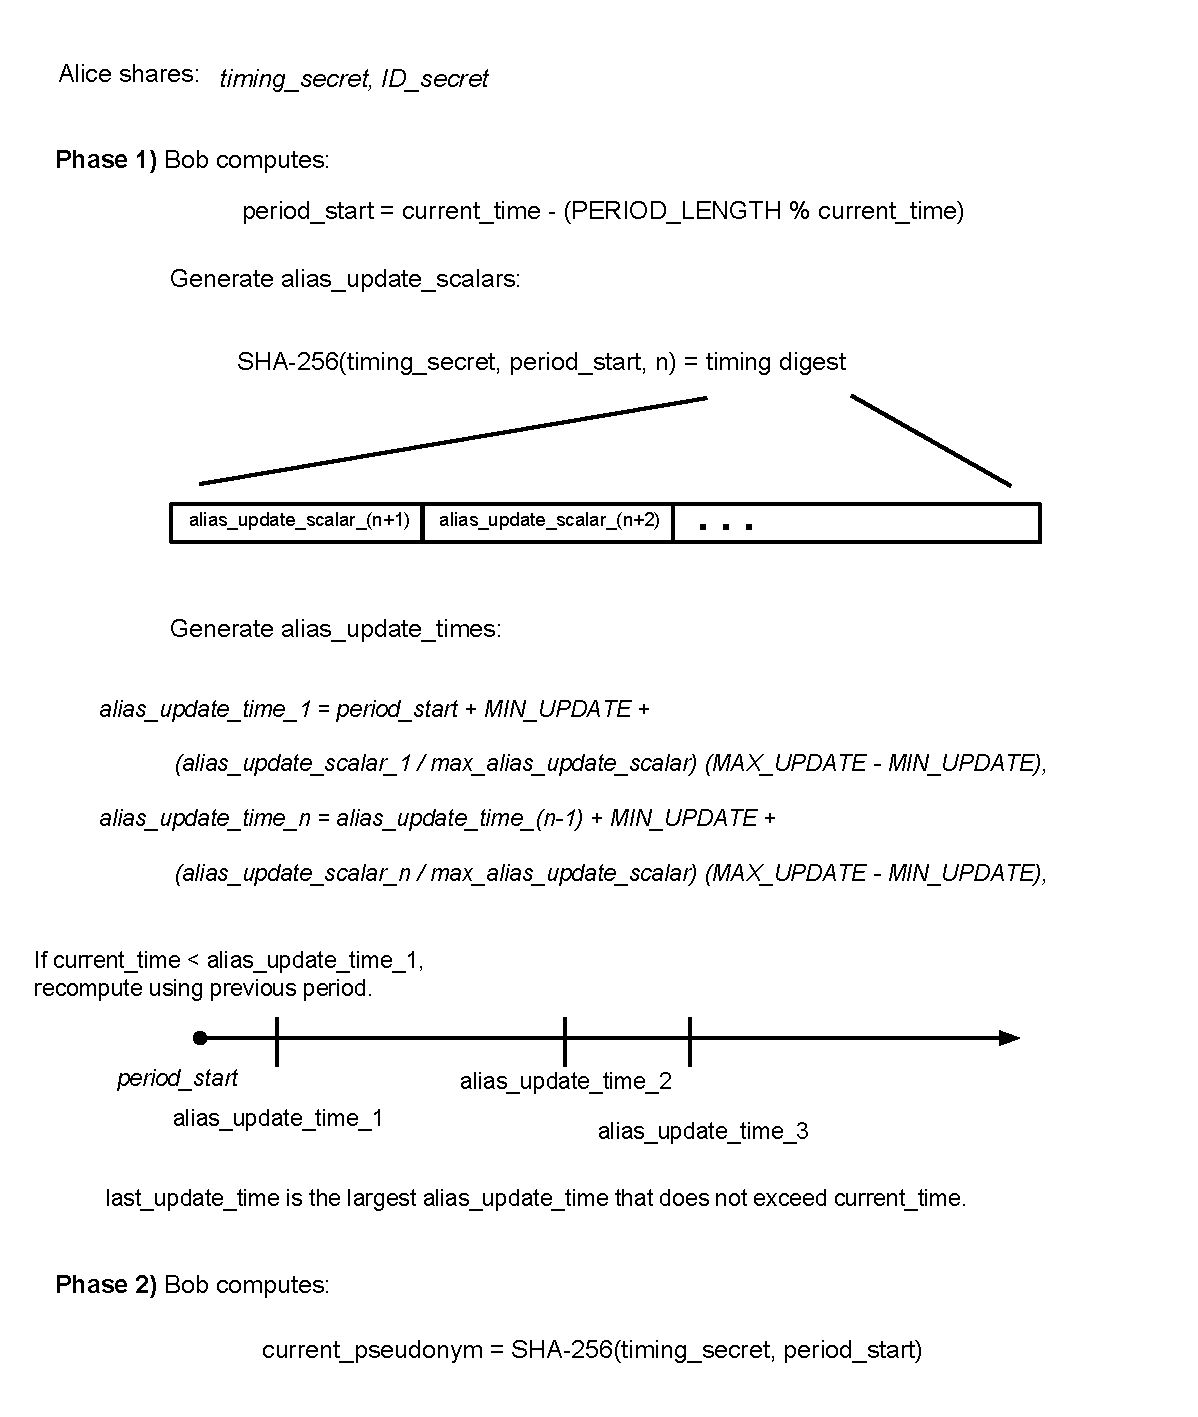
\includegraphics[scale=0.7]{GenerateAlias.pdf}
\end{figure}

\end{document}


